\documentclass[12pt,twoside,singlespace]{article}
%\usepackage{lgrind}
\pagestyle{plain}

\usepackage{array, paralist, enumerate, amsmath, amsthm, amsfonts, amssymb, color, mathrsfs,comment}
%\usepackage{times}
\usepackage{geometry}
\usepackage{framed}
\usepackage{hyperref}
\usepackage{graphicx}
\usepackage{epstopdf}

\usepackage{tikz}
\usepackage{tkz-graph}
\usetikzlibrary{arrows,%
                shapes,positioning}

\definecolor{DarkBlue}{rgb}{0,0,0.8} 
\definecolor{DarkGreen}{rgb}{0,0.5,0.0} 
\definecolor{DarkRed}{rgb}{0.9,0.0,0.0} 

\usepackage[T1]{fontenc}
\usepackage[latin1]{inputenc}
%\usepackage[inline]{showlabels}

\numberwithin{equation}{section}
\newtheorem{thm}[equation]{Theorem}
\newtheorem{lem}[equation]{Lemma}
\newtheorem{cor}[equation]{Corollary}
\newtheorem{prop}[equation]{Proposition}

\theoremstyle{definition}
\newtheorem{definition}[equation]{Definition}
\newtheorem{ex}[equation]{Example}	
\newtheorem{remark}[equation]{Remark}
\newtheorem{prob}{Problem}

\newcommand{\BB}{\mathbf{B}}
\newcommand{\ZZ}{\mathbf{Z}}
\newcommand{\NN}{\mathbf{N}}
\newcommand{\RR}{\mathbf{R}}
\newcommand{\QQ}{\mathbf{Q}}
\newcommand{\CC}{\mathbf{C}}
\newcommand{\FF}{\mathbf{F}}
\newcommand{\N}{N}
\newcommand{\po}[2]{\mathfrak{po}^{#1|#2}}
\newcommand{\on}{\operatorname}
\newcommand{\ra}{\rightarrow}
\newcommand{\ul}{\underline}
\newcommand{\ol}{\overline}
\newcommand{\nin}{\noindent}

\newcommand{\simple}{\text{simple}}
\newcommand{\Img}{\on{Im}}
\newcommand{\con}{\on{Con}}
\newcommand{\dash}{\on{Dash}}

\geometry{verbose,letterpaper,tmargin=1in}

\newcommand{\Q}{\overline{q}}
\newcommand{\w}{\on{weight}}

\newcommand{\val}{\on{Val}}
\newcommand{\smon}{\mathbf{SMon}}
\newcommand{\clif}{\on{clif}}
\newcommand{\cl}{\mathbf{Cl}}
%\newcommand{\mov}[2]{\on{mov}_{#2}(#1)}
\newcommand{\inc}{\on{inc}}
\newcommand{\cut}[4]{#1 = #2 \amalg_{#4} #3}
\newcommand{\cutr}[3]{#1 \amalg_{#3} #2}
%\newcommand{\piece}[3]{#1(#2|#3)}
\newcommand{\piece}[3]{#1_{#3}}
\newcommand{\wt}{\on{wt}}

\newcommand{\com}[1]{\textcolor{red}{$[\star \star \star$ #1 $\star \star \star]$}}

%%%%%%%%%%%%%%%%%%%%%%%%%%%%%% LyX specific LaTeX commands.
%% Bold symbol macro for standard LaTeX users
\providecommand{\boldsymbol}[1]{\mbox{\boldmath $#1$}}

%%%%%%%%%%%%%%%%%%%%%%%%%%%%%% User specified LaTeX commands.
\renewcommand{\vec}[1]{\mathbf{#1}}

%\renewcommand{\labelenumi}{(\alph{enumi})}
%\renewcommand{\labelenumii}{(\roman{enumii})}

%\usepackage{babel}

\title{Study of lifting of 1D adinkras to 2D}
\author{Kevin Iga and Yan X Zhang}

\begin{document}

\pagestyle{plain}

\maketitle

\section{Definitions}

\subsection{$1$-d Adinkras}

Let $V(A)$ be the vertices of $A$.

Recall that a $1$-d adinkra $A$ has a rank function $g: V(A) \rightarrow \ZZ$ (making it into a graded poset). Let $V(A, r)$ be the vertices of $A$ with rank $r$. We will assume $0$ to be the lowest rank in the support of $g$.

Recall that a $1$-d adinkra has a code $L(A)$, which is necessarily doubly-even. The code has parameters $(n,k)$, where $n$ is the number of coordinates and $k$ is the dimensions of the code. In this situation, the vertices of $A$ are labeled by cosets $\{0,1\}^n + L(A)$, so $|V(A)| = 2^{n-k}$.

\subsection{$2$-d Adinkras}

If I read Tristan's stuff right, we can completely translate the combinatorial rules to: a \emph{2-d adinkra} (of dimension $(p,q)$) is a finite simple connected graph $A$ such that:
\begin{itemize}
\item It is an $1$-d adinkra (with the associated ranking, dashing, etc.).
\item It has two color sets $C_L$ and $C_R$, with $|C_L| = p$ and $|C_R| = q$, where the colors in $C_L$ are called \emph{left-moving} and the colors in $C_R$ are called \emph{right-moving}.'' We will slightly abuse notation from now on, saying that an edge is \emph{left-moving} if it has a left-moving color, for example.
\item A coherence condition: for any cycle, we imagine the following sum: going up (here ``up'' comes from the grading we have from the engineering dimension in our ranking for the $1$-d adinkra) a left-moving edge adds $-1$, and going up a right-moving edge adds $1$; going down the edges give contributions with opposite signs. The sum of this around any cycle must be $0$. (in particular, this rules out things like ambidextrous bow-ties)
\end{itemize} 

Assuming I interpreted these rules correctly, now I can do combinatorics without needing any physics.

\section{Structure Theorems}

\subsection{Bigrading}

The first structural fact we can impose is a bi-grading that is compatible with the grading we already have from the $1$-d adinkra structure, in the sense that the $1$-d grading is simply one of the coordinates of our bi-grading.

\begin{prop}
A $1$-d adinkra with color set $C_L \cup C_R$ can be extended to a $2$-d adinkra with left- and right-moving colors $C_L$ and $C_R$ if and only if the $1$-d adinkra has a \emph{bigrading} to $\ZZ^2$ consistent with $C_L$ and $C_R$; this is a map $g: V \rightarrow \ZZ^2$ such that all left-moving edges correspond to displacements of $(0, 1)$ and right-moving edges correspond to displacements of $(1, 0)$.
\end{prop}

\begin{proof}
\com{todo}
\end{proof}

\begin{comment}
This grading allows us to define the notation $V(A, (x,y))$, which is the set of vertices of $A$ of grading $(x,y) \in \ZZ^2$. We will also use the notation $V(A, r)$ to similarly refer to vertices of $A$ of grading $r \in \ZZ$ when referring to $1$-d adinkras, which will come up in our study. Notice that when we consider a $2$-d adinkra as a $1$-d adinkra, we have the relation
\[
V(A,r) = \cup_{x + y = r} V(A, (x,y)).
\]
\end{comment}

A really important consequence of having a bigrading is that we get to ``complete the square'' with the following Corollary:

\begin{cor}
\label{cor:square}
In a $2$-d adinkra, suppose we have a path $(x, y \pm_1 1) \rightarrow (x, y) \rightarrow (x \pm_2 1, y)$, where each $\pm_i$ corresponds to a choice of sign, the first and the last vertices are connected to $(x \pm_2 1, y \pm_1 1)$ via the corresponding colors in a square.
\end{cor}
\begin{proof}
Because we have an ($1$-d) adinkra, the two edges in this path correspond to two different colors (WLOG $1$ and $2$ in order) respectively, and if we use the colors $2$ and $1$ in order we must also reach $(x \pm_2 1, y)$ from $(x, y \pm_1 1)$. Because left-moving colors only correspond to $y$-axis moves in the $\ZZ^2$ bigrading, and right-moving colors only correspond to $x$-axis moves, the first move must have displacement $(\pm_2 1, 0)$ and the second move must have displacement $(0, \pm_1)$. This is exactly equivalent to the statement.
\end{proof}

\subsection{Rectangle}

Let the \emph{support} of a $2$-d adinkra (and/or its bigrading function $g$) be defined as the range of $g$, its bigrading function. Now, we show that the support of $2$-d adinkra must form a rectangle in $\ZZ^2$. In this and the following sections, it helps to have some standard assumptions:

\begin{itemize}
\item Recall that any $1$-d adinkra has vertices labeled by equivalence classes of $\ZZ_2^n$ by some $(n,k)$ doubly-even code $L$. We will refer to vertices by these equivalence classes (or their representatives). We use the notation $(v_1, \ldots, v_n)$ and $(v_1 v_2 \cdots v_n)$ interchangeably.
\item Without loss of generality, let our color set $C_L \cup C_R = \{1,2,\ldots, n\}$, with $C_L = \{1, 2, \ldots, p\}$ and $C_R = \{p+1, p+2, \ldots, p+q=n\}$. We now identify these $n$ elements with the $n$ indices of the vertices thinking of them as the indices of $\ZZ_2^n$. For all $i \in C_L \cup C_R$, define the map $q_i$ that takes a vertex $v$ and returns the unique vertex joined to $v$ by an edge of color $i$. So if $v = (v_1, \ldots, v_n)$, $q_i(v) = (v_1, cdots, v_{i-1}, 1-v_i, v_{i+1}, \cdots, v_n)$. Note that $q_i^2(v) = v$.
\item We will always define $\overline{0}$ to be the vertex corresponding to the equivalence class of $(00\cdots0)$. We will also assume that $g(\overline{0}) = (0,0)$. 
\end{itemize}

For every vertex pair $(v,w)$ in our $2$-d adinkra, there exist (many) paths from $v$ to $w$. Ignoring the dashings for now, let the sequence of colors on any path be called a \emph{color sequence} for the path. So, for example, in a chromotopology corresponding to the unique trivial $(4,0)$ code, the path with color sequence $(3,2,1,1)$ carries $\overline{0} = 0000$ to $0010$, $0110$, $1110$, and finally $0110$. Note that a color sequence $(i_1, i_2, \ldots, i_k)$ sends $v$ to $q_{i_k} q_{i_{k-1}} \cdots q_{i_1} (v)$.

Now, define a map $s$ that takes a color sequence and returns an element of $V = \{0,1\}^n$ where the $i$-th element is the number of times (modulo $2$) that color $i$ appears in the sequence. For example, $s(3,2,1,1) = 0110$. Note that $s(d)$ will return (a member of the equivalence class of) the bitstring obtained by applying the sequence $d$ to $\overline{0}$.  In particular that we may permute a sequence from $d = (d_n)$ to $d' = (d_n')$ without changing the result of $s$. 

The previous work on $1$-d adinkras states that if we start at any vertex, following two paths with color sequences $d$ and $d'$ must end up at the same resulting vertex if and only if $s(d) = s(d') \pmod{L}$. Let $l(d)$ be a rearrangement of $d$ that moves all the left-moving colors to the beginning, and let $r(d)$ be a rearrangement of $d$ that moves all the right-moving colors to the beginning. Thus, suppose $p = q = 2$, we have $l((3,2,1,1)) = (2,1,1,3)$ and $r((3,2,1,1)) = (3,2,1,1)$. We always have $s(l(d)) = s(r(d))$ in general, since $l(d)$ and $r(d)$ are just permutations of each other.

\begin{prop}
\label{prop:rectangle-completion}
Suppose we have any path from $(x,y)$ to $(v,w)$ in a $2$-d adinkra $A$; then the vertices $(x,w)$ and $(v,y)$ are in $A$'s support.
\end{prop}
\begin{proof}
Let this path take color sequence $d$. $l(d)$ and $r(d)$ must both end up at $(v,w)$, but $l(d)$ only changes along the $y$-axis in the first part of moves that only use left-moving colors, so it must end up at coordinate $(x,w)$ to be able to end up at $(v,w)$ (since it can only use right-moving / $x$-axis colors afterwards). Using the same argument for $r(d)$ shows we must end up in $(v,y)$ at some point in the path.
\end{proof}

\begin{cor}
\label{cor:rectangle}
The support of a $2$-d adinkra is exactly some $k \times l$ rectangle. In other words, the set of points in $\ZZ^2$ in the range of $g$, the bigrading map, can be taken to the set of points $(x,y)$, $0 \leq x < l$, $0 \leq y < k$.
\end{cor}
\begin{proof}
If the support is not a rectangle, then there must be some coordinates $(x,y)$ and $(v,w)$ in the support such that one of the other two diagonal coordinates are missing. This violates Proposition~\ref{prop:rectangle-completion}.
\end{proof}

\subsection{Factored by the boundary}

It is fairly neat that the vertices of a $2$-d adinkra $A$ line up nicely in a rectangle. We now show that there is even more regularity in its structure. In particular, its many edges come in identical clumps. Let $A_L$ (resp. $A_R)$ be the subgraphs of $A$ induced by left-moving (resp. right-moving) edges of $A$. %

\begin{lem}
\label{lem:kevin-translate-component}
If $X$ is a connected component of $A_L$ and $i$ is a right-moving color, then $q_i(X)$ is the vertex set of a connected component of $A_L$. The analogous statement for $A_R$ also holds.
\end{lem}
\begin{proof}
Given two vertices $q_i(x)$ and $q_i(x')$ in $q_i(X)$, we know that $x$ and $x'$ are in $X$. Since $X$ is connected in $A_L$, there is a path with left-moving colors from $x$ to $x'$. This means 
\[
x' = q_{j_1}q_{j_2}\cdots q_{j_k} x,
\]
so
\[
q_i (x') = q_i q_{j_1} q_{j_2} \cdots q_{j_k} (x) = q_{j_1} q_{j_2} \cdots q_{j_k} q_i (x),
\]
meaning $q_i(x')$ and $q_i(x)$ are connected in $A_L$. The converse is equally easy.
\end{proof}

\begin{prop}
\label{prop:kevin}
All disconnected components in $A_L$ (and respectively $A_R$) are isomorphic as graded posets.
\end{prop}
\begin{proof}
Let $X$ and $Y$ be two connected components of $A_L$. Pick vertices $x \in X$ and $y \in Y$. Since $A$ is connected, there is a path from $x$ to $y$ in $A$. Reorder the path so that the right-moving edges occur before the left-moving edges. Since the left-moving edges stay in $Y$, the right-moving edges alone take $x$ to a vertex $y' \in Y$. By Lemma~\ref{lem:kevin-translate-components}, each such edge puts us in a new connected component isomorphic to $X$, so $X$ is isomorphic to $Y$. They are all isomorphic as graded posets since translating via right-moving colors does not change the $y$-coordinate of the grading.
\end{proof}

%Let the \emph{left boundary} $B_L(A)$ and \emph{right boundary} $B_R(A)$ of the rectangle be the subgraphs of $A$ induced by vertices of $A$ that occur at the sets $\{(i,0) | 0 \leq i < l \}$ and $\{(0, j) | 0 \leq j < k \}$ respectively. It helps to picture the normal Cartesian plane rotated $45$ degrees counterclockwise, because then adjectives refer to the direction of ``movement'': this way, the left boundary corresponds to the lower-left vertices in the support rectangle and the right boundary corresponds to the lower-right vertices.

With all this redundancy, what is the minimal amount of information required for us to understand a $2$-d adinkra? It turns out we just need a single connected component for each direction.

\begin{thm}
\label{thm:connected component factorization}
Consider the vertex $\overline{0} \in A$. Let the connected component of $A_L$ (resp. $A_R$) that $\overline{0}$ belongs to be labeled $A_L^0$ (resp. $A_R^0$). The adinkra $A$ is uniquely determined by $A_L^0 \cup A_R^0$.
\end{thm}
\begin{proof}
Consider the color sequence $d$ of any path from $v$ to a vertex $u$ in $B_R(A)^v$. Pick any left-moving color $c$. Examine the sequence $cd$. Corollary~\ref{cor:square} will force the $cd_1$ to end with the same $x$-axis displacement as $d_1$, $cd_1d_2$ to end with the same $x$-axis displacement as $d_1d_2$, etc. so inductively any color sequence $cd$ will end with the same $x$-axis displacement as $d$. Using induction, we get that for every one of the elements $u$ of $B_L(A)^0$, the right-moving ($x$-axis) colors starting at $u$ forms a copy $B_R(A)^v$ whose $x$-axis positions are forced by the right boundary. 

The key observation is that every element $u$ of the adinkra can be reached starting at $v$ via moving to an element of the left boundary and then using only right-moving moves (i.e. by taking $l(d)$ for any color sequence $d$ that goes from $v$ to $u$). Because of the discussion in our previous paragraph, $B_R(A)^v$ and $B_L(A)^v$ uniquely tell us how to obtain the coordinates of $u$.
\end{proof}

\begin{figure}[htb]
\begin{center}

\begin{tabular}{c|c}
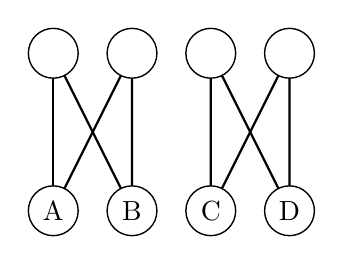
\begin{tikzpicture}[scale=0.10]
%\SetVertexNormal
\SetUpEdge[labelstyle={draw}]
\Vertex[x=0,y=0]{A}
\Vertex[x=10,y=0]{B}
\Vertex[x=20,y=0]{C}
\Vertex[x=30,y=0]{D}
\SetVertexNoLabel
\Vertex[x=0,y=20]{E}
\Vertex[x=10,y=20]{F}
\Vertex[x=20,y=20]{G}
\Vertex[x=30,y=20]{H}
\Edges(A, F, B, E, A)
\Edges(C, H, D, G, C)
\end{tikzpicture}
&
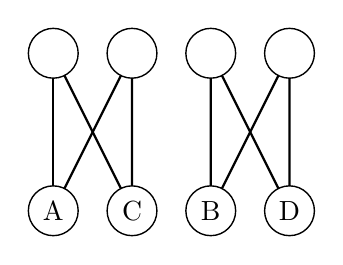
\begin{tikzpicture}[scale=0.10]
%\SetVertexNormal
\SetUpEdge[labelstyle={draw}]
\Vertex[x=0,y=0]{A}
\Vertex[x=10,y=0]{C}
\Vertex[x=20,y=0]{B}
\Vertex[x=30,y=0]{D}
\SetVertexNoLabel
\Vertex[x=0,y=20]{E}
\Vertex[x=10,y=20]{G}
\Vertex[x=20,y=20]{F}
\Vertex[x=30,y=20]{H}
\Edges(A, G, C, E, A)
\Edges(B, H, D, F, B)
\end{tikzpicture}
\end{tabular}
%\includegraphics[scale=0.5]{4cubefold}
\caption{Tensoring the two adinkras here with the following identification gives a non-disconnected adinkra with 16 vertices. \label{fig:disconnected}}
\end{center}
\end{figure}


We will worry less about exact rankings right now with the following construction: for an $1$-d adinkra $A$ let $\val(A)$ be the valise form of $A$. For any $2$-d adinkra $A$ with boundary pair $(B_L(A), B_R(A))$, the adinkra defined by the boundary pair $(\val(B_L(A)), \val(B_R(A)))$ is again a $2$-d adinkra. We will abuse notation and call this new adinkra $\val(A)$, and call such an adinkra (i.e. where the rectangle is a $2 \times 2$ square) a \emph{valise} ($2$-d) adinkra. We seek the following theorem, which is very similar to Theorem~\ref{thm:boundary factorization}

\begin{cor}
\label{cor:valise factorization}
A valise $2$-d adinkra $A$ of type $(n,k)$ is uniquely determined by $B_L(A)$, $B_R(A)$, and an identification of $V(B_L(A), 0)$ and $V(B_R(A), 0)$. Furthermore, $|B_L(A)| = |B_R(A)| = 2^{n-k-1}$.
\end{cor}



\begin{figure}[htb]
\begin{center}

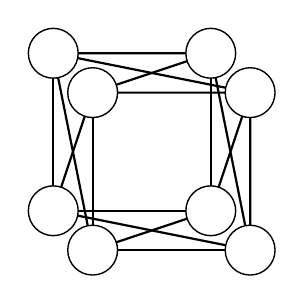
\begin{tikzpicture}[scale=0.10]
%\SetVertexNormal
\SetVertexNoLabel
\SetUpEdge[labelstyle={draw}]
\Vertex[x=0,y=0]{A}
\Vertex[x=-5,y=5]{H}
\Vertex[x=0,y=20]{C}
\Vertex[x=-5,y=25]{B}
\Vertex[x=15,y=5]{D}
\Vertex[x=20,y=0]{E}
\Vertex[x=20,y=20]{G}
\Vertex[x=15,y=25]{F}
\Edges(A,B,G)
\Edges(B,H,C)
\Edges(G,D)
\Edges(C,A,D,H,E,A)
\Edges(D,F,C,G,E,F,B)
\end{tikzpicture}
\caption{This is a tight valise which cannot be lifted.\label{fig:tight valise}}
\end{center}
\end{figure}

\begin{prob}
What are all the $2$-d adinkras $A$ with the same valise adinkra $\val(A)$? Not all lifts are possible. For example, the adinkra in Figure~\ref{fig:tight valise} cannot be lifted to any non-valise form!
\end{prob}

\section{Quotienting}



Define a \emph{even-split doubly-even (ESDE) code} to be a doubly-even code isomorphic to a direct sum $C_L \oplus C_R$ of even codes. It was proved \cite{blah} that $1$-d adinkras are ismorphic to quotienting the hamming cube $H^n$ by a doubly-even code, so any adinkra $A$ has a well-defined associated code $L(A)$ that is uniquely determined by just the graph structure of the adinkra.

Our goal is to show
\begin{thm}
The image of $C$ of the set of $2$-d adinkras are exactly the ESDE codes.
\end{thm}

This answers a conjecture of H\"{u}bsch \cite{}.

To do this we need to show two things:

\begin{prop}
Any valise $2$-d adinkra $A$ has $L(A)$ equal to a ESDE code.
\end{prop}
\begin{proof}

Note that the automorphism group of the adinkra is defined by the basepoint.

TODO
\end{proof}

\begin{prop}
Any ESDE code defines a valise $2$-d adinkra $A$.
\end{prop}
\begin{proof}
TODO
\end{proof}

Here are some other problems:
\begin{prob}
Given two valise $1$-d adinkras $B_L(A)$ and $B_R(A)$ of equal size, what identifications of $V(B_L(A), 0)$ and $V(B_R(A), 0)$ are possible?
\end{prob}
\begin{proof}
Data: if we have $\{0,1\} \cup \{2,3\}$ on one side, the other side must be $\{0,2\} \cup \{1, 3\}$.
\end{proof}

\com{There are two kinds of quotienting that we can think of: one quotient is directly quotienting the mega hypercube adinkra by a ESDE code; one quotient is given the valise adinkra with associated $B_L(A)$, $B_R(A)$ each with $2^{d+1}$ vertices, the necessary $d$-dimensional quotienting that occurs when we naively tensor the two parts (which gives $2^{2d}$ vertices in each corner, for $2^{2d+2}$ total vertices, when in the end we just want $2^{d+2}$ vertices.}

\section{ESDE Codes}

In this section, we classify all ESDE codes.

\com{TODO!}


\begin{comment}
\section{Other stuff}
\begin{center}
\begin{tabular}{ccc}
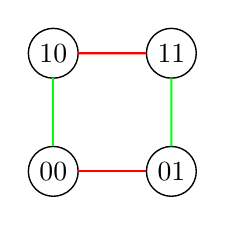
\begin{tikzpicture}[scale=0.15]
\SetUpEdge[labelstyle={draw}]
\Vertex[x=10,y=10]{11}
\Vertex[x=0,y=10]{10}
\Vertex[x=10,y=0]{01}
\Vertex[x=0,y=0]{00}
\Edge[color=green](00)(10)
\Edge[color=red](00)(01)
\Edge[color=red](10)(11)
\Edge[color=green](01)(11)
\end{tikzpicture}
&
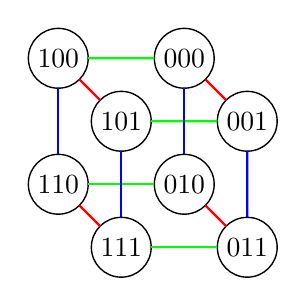
\begin{tikzpicture}[scale=0.08]
%\SetVertexNormal
\SetUpEdge[labelstyle={draw}]
\Vertex[x=0,y=0]{111}
\Vertex[x=20,y=0]{011}
\Vertex[x=0,y=20]{101}
\Vertex[x=20,y=20]{001}
\Vertex[x=-10,y=10]{110}
\Vertex[x=10,y=10]{010}
\Vertex[x=-10,y=30]{100}
\Vertex[x=10,y=30]{000}
\Edge[color=red](100)(101)
\Edge[color=red](000)(001)
\Edge[color=red](010)(011)
\Edge[color=red](110)(111)
\Edge[color=green](000)(100)
\Edge[color=green](001)(101)
\Edge[color=green](010)(110)
\Edge[color=green](011)(111)
\Edge[color=blue](000)(010)
\Edge[color=blue](001)(011)
\Edge[color=blue](100)(110)
\Edge[color=blue](101)(111)
\end{tikzpicture}
&
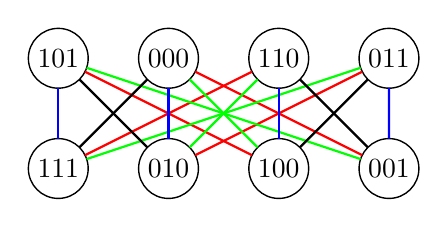
\begin{tikzpicture}[scale=0.14]
\SetUpEdge[labelstyle={draw}]
\Vertex[x=0,y=0]{111}
\Vertex[x=0,y=10]{101}
\Vertex[x=10,y=0]{010}
\Vertex[x=10,y=10]{000}
\Vertex[x=20,y=10]{110}
\Vertex[x=30,y=10]{011}
\Vertex[x=20,y=0]{100}
\Vertex[x=30,y=0]{001}
\Edge[color=red](100)(101)
\Edge[color=red](000)(001)
\Edge[color=red](010)(011)
\Edge[color=red](110)(111)
\Edge[color=green](000)(100)
\Edge[color=green](001)(101)
\Edge[color=green](010)(110)
\Edge[color=green](011)(111)
\Edge[color=blue](000)(010)
\Edge[color=blue](001)(011)
\Edge[color=blue](100)(110)
\Edge[color=blue](101)(111)
\Edge[color=black](100)(011)
\Edge[color=black](000)(111)
\Edge[color=black](010)(101)
\Edge[color=black](110)(001)
\end{tikzpicture}
\end{tabular}
\end{center}

An \emph{adinkra} is a chromotopology with the following properties:
\begin{enumerate}
\item \emph{ranked}: we give $A$ additional structure of a ranked poset; this is a function $h\colon V(A) \rightarrow \ZZ$ such that $|h(x) - h(y)| = 1$ for edges $(x,y) \in E(A)$. 
\item \emph{dashed}: we give an \emph{odd dashing}; this is a function $d\colon E(A) \rightarrow \ZZ_2$ such that for all $2$-colored $4$-cycles $\textbf{c}$, $\sum_{e \in \textbf{c}} d(e) = 1 \in \ZZ_2$. 
\end{enumerate}

\begin{center}
\begin{tabular}{cc}
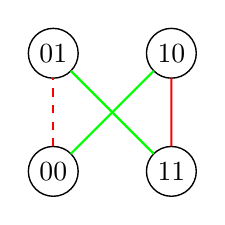
\begin{tikzpicture}[scale=0.15]
\SetUpEdge[labelstyle={draw}]
\Vertex[x=10,y=0]{11}
\Vertex[x=10,y=10]{10}
\Vertex[x=0,y=10]{01}
\Vertex[x=0,y=0]{00}
\Edge[color=green](00)(10)
\Edge[color=red, style=dashed](00)(01)
\Edge[color=red](10)(11)
\Edge[color=green](01)(11)
\end{tikzpicture}
& 
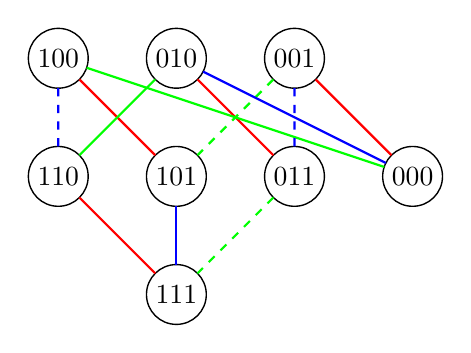
\begin{tikzpicture}[scale=0.15]
%\SetVertexNormal
\SetUpEdge[labelstyle={draw}]
\Vertex[x=0,y=0]{111}
\Vertex[x=0,y=10]{101}
\Vertex[x=0,y=20]{010}
\Vertex[x=20,y=10]{000}
\Vertex[x=-10,y=10]{110}
\Vertex[x=10,y=10]{011}
\Vertex[x=-10,y=20]{100}
\Vertex[x=10,y=20]{001}
\Edge[color=red](100)(101)
\Edge[color=red](000)(001)
\Edge[color=red](010)(011)
\Edge[color=red](110)(111)
\Edge[color=green](000)(100)
\Edge[color=green, style=dashed](001)(101)
\Edge[color=green](010)(110)
\Edge[color=green, style=dashed](011)(111)
\Edge[color=blue](000)(010)
\Edge[color=blue, style=dashed](001)(011)
\Edge[color=blue, style=dashed](100)(110)
\Edge[color=blue](101)(111)
\end{tikzpicture}
\\
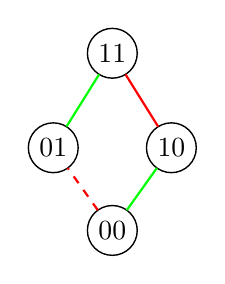
\begin{tikzpicture}[scale=0.15]
\SetUpEdge[labelstyle={draw}]
\Vertex[x=5,y=15]{11}
\Vertex[x=10,y=7]{10}
\Vertex[x=0,y=7]{01}
\Vertex[x=5,y=0]{00}
\Edge[color=green](00)(10)
\Edge[color=red, style=dashed](00)(01)
\Edge[color=red](10)(11)
\Edge[color=green](01)(11)
\end{tikzpicture}
&
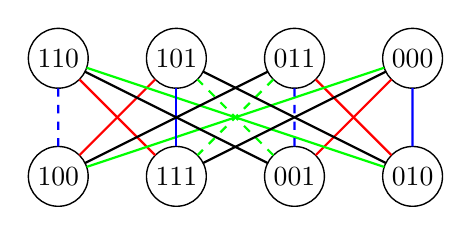
\begin{tikzpicture}[scale=0.15]
%\SetVertexNormal
\SetUpEdge[labelstyle={draw}]
\Vertex[x=0,y=0]{111}
\Vertex[x=0,y=10]{101}
\Vertex[x=20,y=0]{010}
\Vertex[x=20,y=10]{000}
\Vertex[x=-10,y=10]{110}
\Vertex[x=10,y=10]{011}
\Vertex[x=-10,y=0]{100}
\Vertex[x=10,y=0]{001}
\Edge[color=red](100)(101)
\Edge[color=red](000)(001)
\Edge[color=red](010)(011)
\Edge[color=red](110)(111)
\Edge[color=green](000)(100)
\Edge[color=green, style=dashed](001)(101)
\Edge[color=green](010)(110)
\Edge[color=green, style=dashed](011)(111)
\Edge[color=blue](000)(010)
\Edge[color=blue, style=dashed](001)(011)
\Edge[color=blue, style=dashed](100)(110)
\Edge[color=blue](101)(111)
\Edge[color=black](100)(011)
\Edge[color=black](000)(111)
\Edge[color=black](010)(101)
\Edge[color=black](110)(001)
\end{tikzpicture}
\end{tabular}
\end{center}

Call the corresponding chromotopologies \emph{adinkraizable.} As we see above, $I^2$, $I^3$, and $K_{4,4}$ are adinkraizable.

\section{Chromotopologies are Quotients}

An  $(n,k)$-\emph{code} is a $k$-dimensional $\ZZ_2$-subspace of $\ZZ_2^{n}$. There are many interesting families of codes, many of which involve looking at the \emph{weights} (the number of $1$'s) of its codewords. A code is \emph{even} if all its codewords have weight divisible by $2$. A code is \emph{doubly even} if all its codewords have weight divisible by $4$.

We can quotient $I^n$ by a code $L$ by identifying vertices whose difference is in $L$ and edges similarly. The quotient $I^2/\{00, 11\}$:

\begin{center}
\begin{tabular}{ccc}
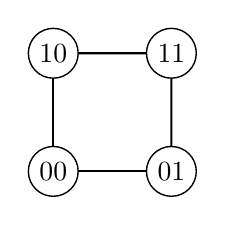
\begin{tikzpicture}[scale=0.15]
\SetUpEdge[labelstyle={draw}]
\Vertex[x=10,y=10]{11}
\Vertex[x=0,y=10]{10}
\Vertex[x=10,y=0]{01}
\Vertex[x=0,y=0]{00}
\Edge[](00)(10)
\Edge[](00)(01)
\Edge[](10)(11)
\Edge[](01)(11)
\end{tikzpicture}
&
becomes
&
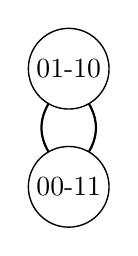
\begin{tikzpicture}[scale=0.15]
%\SetVertexNormal
\SetUpEdge[labelstyle={draw}]
\Vertex[L=00-11, x=0,y=0]{0}
\Vertex[L=01-10, x=0,y=10]{1}
\Edge[style={bend left}](0)(1)
\Edge[style={bend right}](0)(1)
\end{tikzpicture}
\end{tabular}
\end{center}

\begin{theorem}[Z, 2011]
\label{thm:classification}
The following classification holds:
\begin{enumerate}
\item Prechromotopologies are exactly quotients $I^n/L$ for some code $L$. 
\item Chromotopologies are exactly such quotients where $L$ is an even code with no bitstring of weight $2$. 
\item (DFGHIL, 2008) Adinkraizable chromotopologies are exactly such quotients where $L$ is a doubly even code.
\end{enumerate}
\end{theorem}

\begin{framed}
\noindent We can now just label chromotopologies by $(n,k)$-codes! Furthermore, hypercubes are the ``universal'' objects of adinkras.
\end{framed}

For example, the $K_{4,4}$ graph we saw before (the only graph that was not a Hamming cube) is actually $I^4/\{0000,1111\}$! Rich combinatorial problems remain when we try to understand dashings and rankings. 

\begin{table}
\begin{center}$
\begin{array}{|l|l|l|l|}
\hline 
n & \text{dashings} & \text{rankings} & \text{full adinkras}\\ 
\hline
1 & 2 &  2 & 4 \\
2 & 8 & 6 & 48 \\ 
3 & 128 & 38 & 4864 \\ 
4 & 32768 & 990 & 32440320 \\
5 & 2147483648 & 395094 & 848457904422912 \\
\hline
\end{array}
$\end{center}
\label{table:counting cubes}
\caption{Enumeration of dashings, rankings, and full adinkras with chromotopology $I^n$.}
\end{table}

\begin{prob}
What are the number of rankings with the $n$-cubical chromotopology for $n \geq 6$? What about other chromotopologies (quotients of cubes)?
\end{prob}

\begin{prob}
What about for other bipartite graphs? Rankings generalize trivially to all bipartite graphs. There's some interesting potential here. Putting poset structures on graphs is called ``acyclic orientations.'' A result of Stanley is that acyclic orientations has to do with the chromatic polynomial evaluated at $-1$. Well, for square-free graphs (see the following discussion), we have a connection between \emph{graded} poset structures on graphs and chromatic polynomial evaluation at $3$. I suspect there is much more stuff going on here. Why?
\end{prob}

\begin{prob}
Some work by Galvin (\cite{galvin:cube} and \cite{galvin:tori}) has shown the awesome result that "most rankings of the Hamming cube" have a range of <= 5! (he did it in a slightly different language) He also shows asymptotically what the counts are for ranges 2, 3, 4, and 5 actually being realized. Doing the same for quotients of the Hamming cube is interesting (as Galvin himself told me).
\end{prob}

An \emph {squarely generated graph} is a graph whose cycle space is generated by 4-cycles.Note that Hamming cubes and grid graphs are squarely-generated. The following is a very cute result (but not substantial, as people already realized this for Hamming cubes and this is a simple generalization over that case).

\begin{theorem}[Klein-Z, 2012]
If $G$ is a squarely generated graph, then $|R(G)|=\frac{1}{3}\chi_G(3)$.
\end{theorem}

This connects the problem to classical coloring problems and statistical mechanics! (see \cite{lieb:square_ice} and \cite{salas:first}, for example)

\begin{prob}
Recall that adinkras are just quotients $I^n/L$. Is there a nice condition for $I^n/L$ to be squarely generated? (this is probably very easy)
\end{prob}

Let a \emph{discrete Lipschitz function} denote a function $V(G) \rightarrow \ZZ$ such that if $(i,j) \in E(G)$, $|f(i) - f(j)| \leq 1$.

\begin{itemize}
\item We have that the number of discrete Lipschitz functions on $G \times I$ is $2|R(G)|$. 
\item Consider the polytope in $R^{|V(G)|}$ created by $x_i - x_j = \pm 1$ for $(i,j) \in E(G)$, and $x_1 = 0$. The integral points are discrete Lipschitz functions and the vertices are rankings. 
\end{itemize}


\begin{prob}
Understand this polytope? Count its lattice points? Ehrhart theory? It would be fun to just take this polytope as an object and play with it. This is good for "researcher" types since it ties with more modern algebraic combinatorics. The polytope itself can be seen via the angles of "root polytopes", "alcoved polytopes", or hyperplane arrangements. Finding its Ehrhart polynomial may be fun for example. Chris O'Neil (Duke) said it may be fun to attack this problem with LATTE, a computer package for dealing with polytopes. This would be a very hands-on way of playing with this problem and be fairly open-minded (volume, lattice points, vertices, etc. of polytopes are all somewhat connected and possibly fun to count)
\end{prob}

\begin{prob}
Count and/or understand DLFs for adinkras or other graphs? Note DLFs make complete sense for non-bipartite graphs as well! In fact, any of the problems about rankings have an equivalent problem for DLFs. 
\end{prob}

\begin{prob}
In particular, copying Galvin's stuff for DLFs seem like really low-hanging fruit. \cite{peled:flat} has some good work on DLFs.
\end{prob}

\section{Misc. Problems}

These are a bit more open-ended:

\begin{prob} Adinkras basically come out from studying the representations of a particular algebra, but the way we build these graphs apply to other algebras! What happens when we study dashings and rankings of other graphs? They basically generalize Cayley diagrams.
\end{prob}

\begin{prob} (for people with some interest in coding theory and topology) What can we do with this "Stiefel-Whitney classes of codes (see \cite{zhang:thesis}? Do classical coding theory results correspond to cool things in SW-classes? Maybe something with MacWilliams / Gleason's Theorems?
\end{prob}

\begin{prob}
Don't forget that any of these exact enumeration questions may be asked in the light of asymptotic combinatorics. Complexity theory suggests that rankings in particular may be NP-complete (because they are equivalent to 3-colorings in certain cases).
\end{prob}

\section{Motivation}

Roughly, we want to understand off-shell representations of the $N$-extended Poincar\'{e} superalgebra in the $1$-dimensional worldline. This gives us an easy example of a superalgebra to play with. In physics, it is customary to classify things with graphical diagrams (good practice for mathematicians too!) and in a series of papers starting with \cite{d2l:first}, different subsets of the ``DFGHILM collaboration'' (Doran, Faux, Gates, H\"{u}bsch, Iga, Landweber, Miller) have built and extended the machinery of \emph{adinkras}.

For more information, see \cite{zhang:thesis}, my thesis, for most details. My main publication on this is \cite{zhang:adinkras}, which is a subset of the material in my thesis.

\end{comment}

\bibliographystyle{abbrv}
\bibliography{Adinkras}

\end{document}